\begin{frame}{Generative Models}
    \begin{columns}
        \begin{column}{0.5\linewidth}
            \small
            \begin{itemize}
                \item Given observed samples $\vx$, generative models learn the data distribution $p(\vx)$
                \item Examples include:
                      \begin{itemize}
                          \item \acp{gan}
                          \item \acp{vae}
                          \item \acp{nf}
                          \item Diffusion models
                      \end{itemize}
            \end{itemize}
        \end{column}
        \begin{column}{0.5\linewidth}
            \begin{figure}
                \centering
                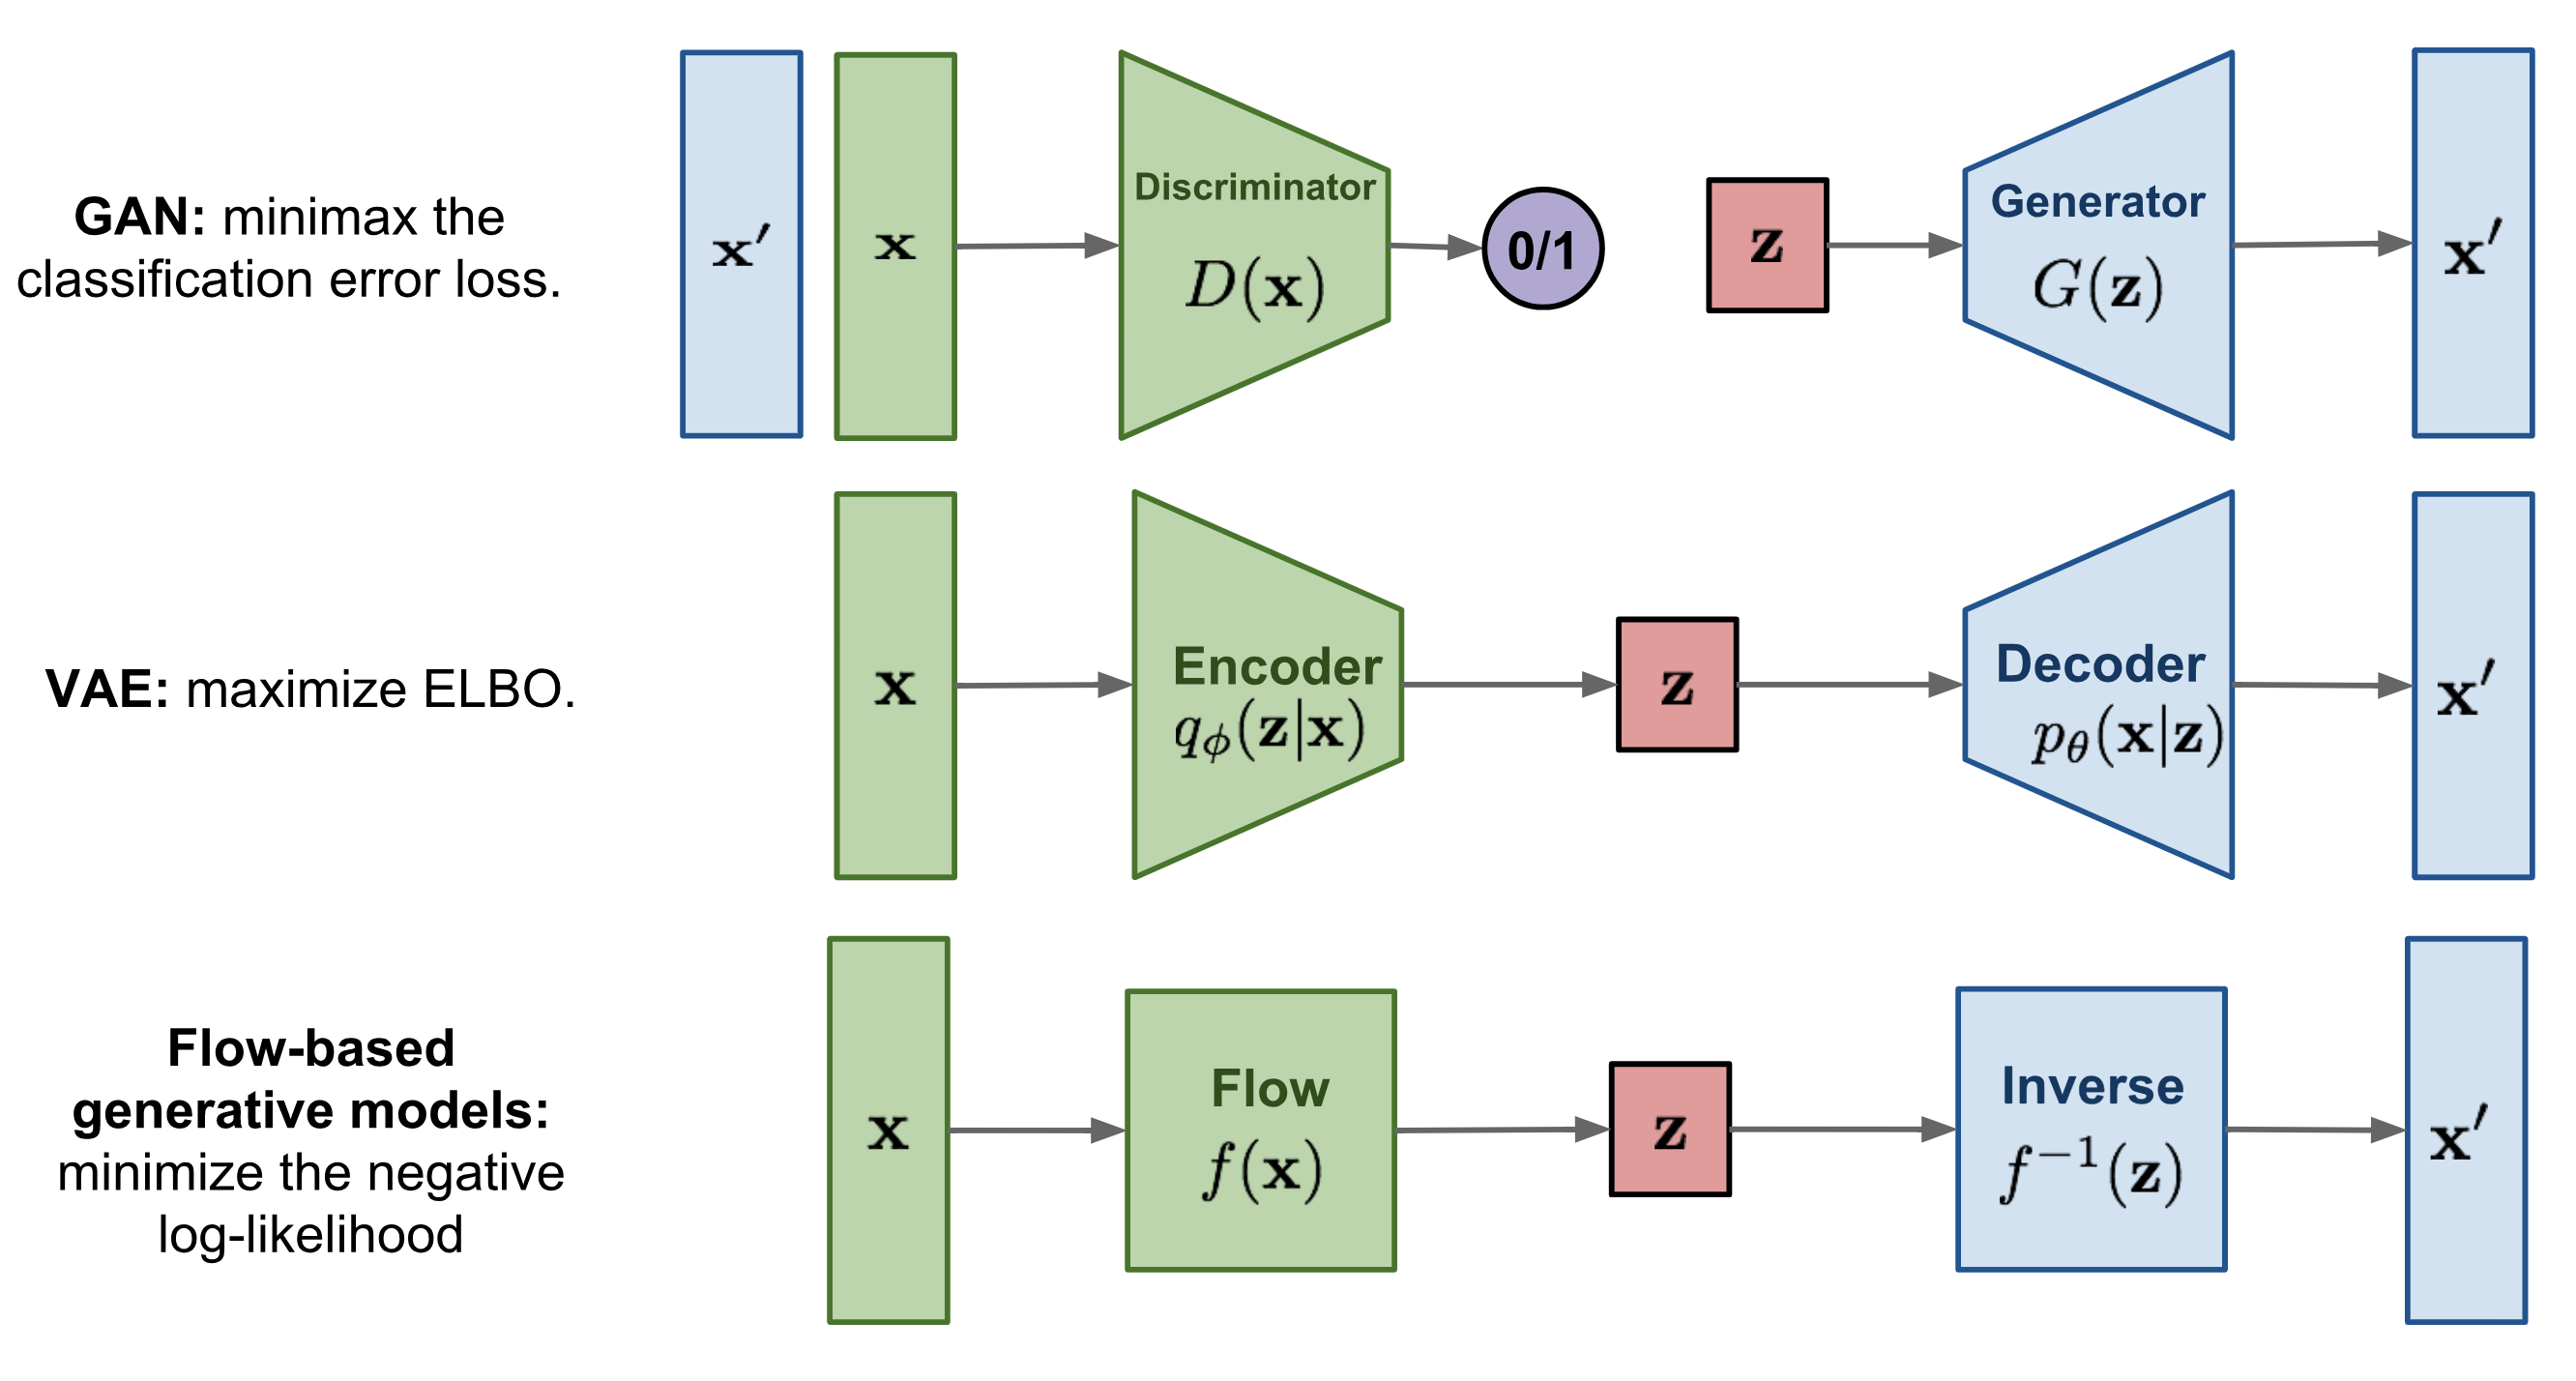
\includegraphics[width=\linewidth]{images/generative_models.png}
            \end{figure}
        \end{column}
    \end{columns}
\end{frame}